\documentclass{article}
\usepackage{graphicx}

\begin{document}

\begin{flushleft}
Contemporary Mathematics\\
Volume 57, 1986
\end{flushleft}







\begin{center}
RECURSIVE ORDERED SETS\\
Henry A. Kierstead
%\maketitle
\end{center}
§ 1 Introduction\\
\indent
Many mathematicians working in finite combinatorics are highly suspicious of infinite sets and structures.   This suspicion does not extend to all infinite structures.   The set of natural numbers with the usual order is considered quite acceptable and, on the whole, so is the set of real numbers with its usual order.   The problems arise when some unusual structure is placed on these sets as in well ordering the real numbers.   Other examples arise from extending theorems about finite structures to theorems about infinite   structures.    Once Dilworth's Theorem has been proven for finite ordered sets it is routine to extend it to infinite ordered sets of finite width,via the Compactness Theorem.   However the resulting structure may be qui te unusual.   The proof only shows the existence of a chain cover; it does not produce the chain cover.   This is the source of the uneasiness in both cases:    The structures whose existence is asserted have not been shown to be available for inspection.\\
\indent
Rather than ignoring these existence results one should go one step further and ask whether there is a satisfactory structure available for inspection. This leads to further questions. What does it mean to be available for inspection? How would you show that there was no satisfactory structure available for inspection? For countable structures these concerns can be made precise and can often be resolved using the theory of recursive (i.e. computable) functions.   The resulting combinatorial theory is the subject of this article, which in particular will'concentrate on antichain covers, chain covers, and realizers of recursive ordered sets.\\
\indent
Let us agree that a structure is available for inspection if it is recursive, where, roughly speaking, a relational structure   P   is recursive if it is recursive, where, roughly speaking, a relational structure P is recursive if\\
\newline
---------------\\
1980 Mathematics Subject Classification. Primary 03D45. supported by ONR grant N00014-85K-0494
\newline

\begin{flushright}
© 1986 American Mathematical Society 0271-4132/86 $1.00 + $.25 per page
\end{flushright}






































% SEKCJA Z OBRAZKAMI
\begin{picture}(100, 100)
%\linethickness{2mm}
\thicklines
\put(0, 0){\circle{5}}
\put(0, -40){\circle{5}}
\put(40, 0){\circle{5}}
\put(40, -40){\circle{5}}
\put(2, -38){\line(1, 1){36}}
\put(0, -2){\line(0, -1){36}}
\put(-38, -2){\line(1, 1){36}}
\put(40, -38){\line(0, 1){36}}
\put(40, -38){\line(1, 1){14}}
\put(160, -40){\circle{5}}
\put(160, 0){\circle{5}}
\put(158, -2){\line(-1, -1){14}}
\put(2, -1){\line(4, -1){156}}
\put(160, -2){\line(0, -1){36}}

\put(100, -20){\circle*{3}}
\put(110, -20){\circle*{3}}
\put(120, -20){\circle*{3}}

\end{picture}

\begin{picture}(100, 100)
\thicklines
\put(0, 0){\circle{3}}
\put(0, -20){\circle{3}}
\put(0, -40){\circle{3}}
\put(0, -60){\circle{3}}
\put(0, -80){\circle{3}}
\put(20, -60){\circle{3}}
\put(20, -80){\circle{3}}
\put(40, -60){\circle{3}}
\put(40, -80){\circle{3}}
\put(40, -100){\circle{3}}
\put(40, -120){\circle{3}}
\put(40, -140){\circle{3}}

\put(0, -2){\line(0, -1){16}}
\put(0, -22){\line(0, -1){16}}
\put(0, -42){\line(0, -1){16}}
\put(0, -62){\line(0, -1){16}}
\put(1, -61){\line(1, -1){18}}
\put(1, -79){\line(1, 1){18}}

\put(21, -61){\line(1, -1){18}}
\put(21, -79){\line(1, 1){18}}

\put(40, -62){\line(0, -1){16}}
\put(40, -82){\line(0, -1){16}}
\put(40, -102){\line(0, -1){16}}
\put(40, -122){\line(0, -1){16}}

\put(-15, -1){$c_1^0$}
\put(-15, -61){$c_1^i$}
\put(-20, -81){$c_1^{i+1}$}
\put(24, -58){\footnotesize y}
\put(24, -84){\footnotesize x}
\put(45, -61){$c_2^{i+1}$}
\put(45, -81){$c_2^i$}
\put(45, -141){$c_2^0$}
\put(14, -137){(b)}


\end{picture}

\newpage
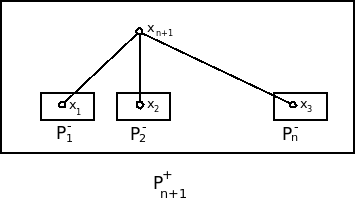
\includegraphics[scale=0.5]{figures/Figure1.png}
\newpage
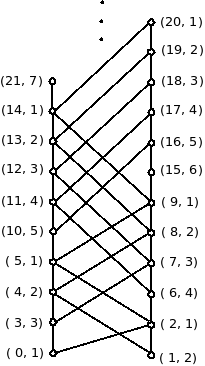
\includegraphics[scale=0.5]{figures/Figure3.png}
\newpage
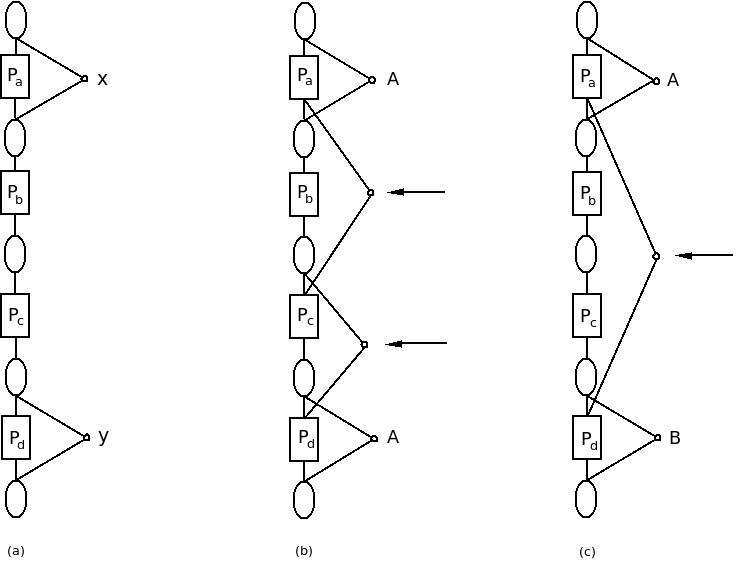
\includegraphics[scale=0.5]{figures/Figure5.png}

\end{document}


